\subsection{TOOL NAME : SLiMFinder}
\vspace{8pt}
\textbf{Running Process} : Online \\ \\
The tool is run on an online server that takes necessary input files and parameters and outputs the motif matches


\subsubsection{Software Link}
The tool can be found at: http://www.slimsuite.unsw.edu.au/servers/slimfinder.php

\vspace{8pt}

\subsubsection{Interface}
\begin{center}
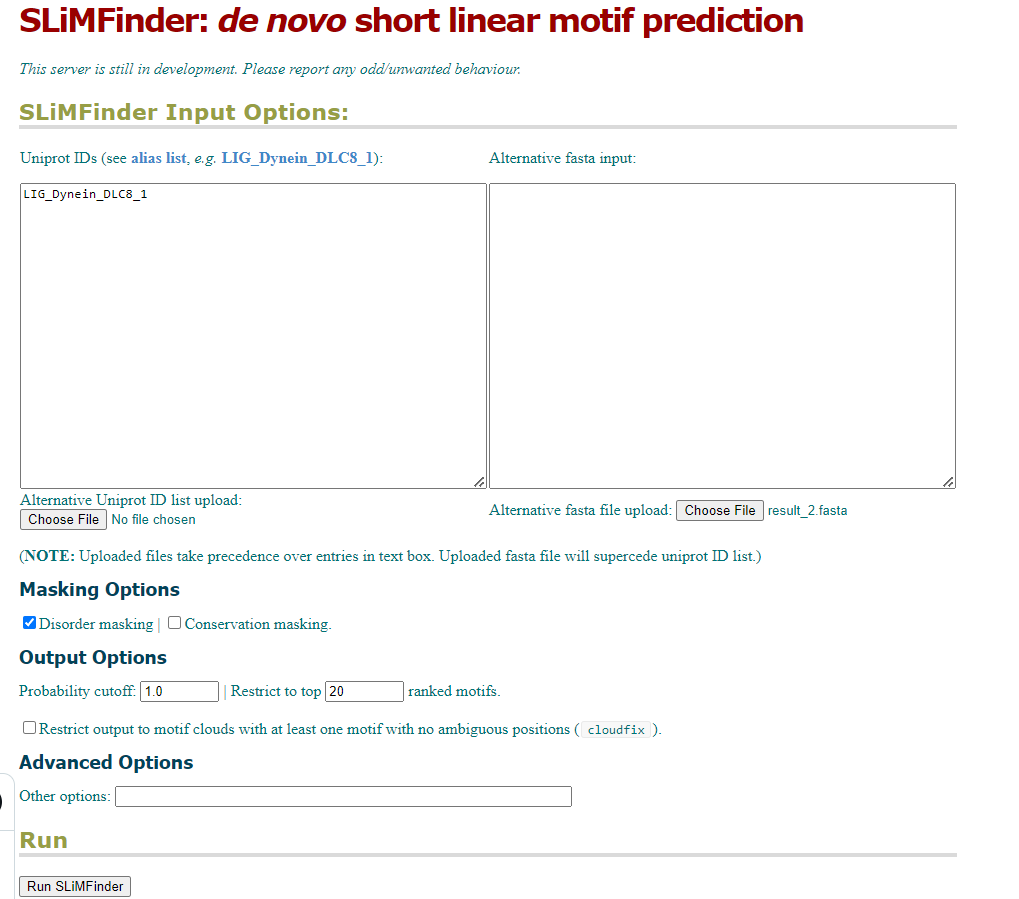
\includegraphics[width=14cm]{images/interface2.png}
\end{center}
\begin{center}
\textbf{SLiMFinder Interface}
\end{center}

\vspace{8pt}

\textbf{Explanation: }Here we set it such that we only take the top 20 ranked motifs of length 20 or less, this means that there can be motifs of lesser length as well.

\\


\subsubsection{Generated Output}
After running SLiMFinder, we find that there are motifs of different length with different start-positions and end-positions. Here we show a portion of the whole output

\vspace{8pt}
\begin{center}
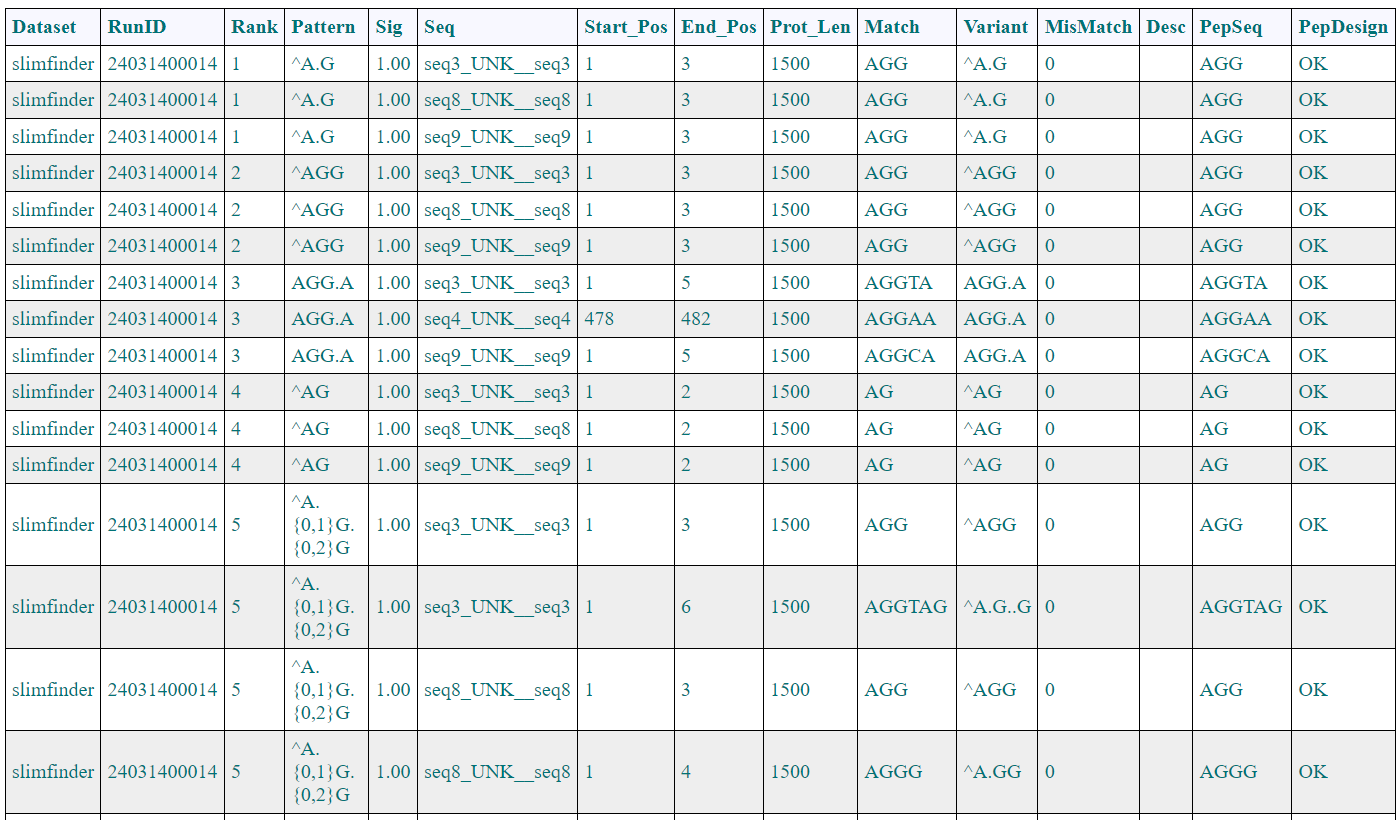
\includegraphics[width=14cm]{images/output2.png}
\end{center}
\begin{center}
\textbf{SLiMFinder Result}
\end{center}
\vspace{8pt}

\subsubsection{Motif Generation}

According to the consensus, a portion of the matched pairs is shown below. They are sorted by rank and also by match percentage. 

\vspace{8pt}
\begin{center}
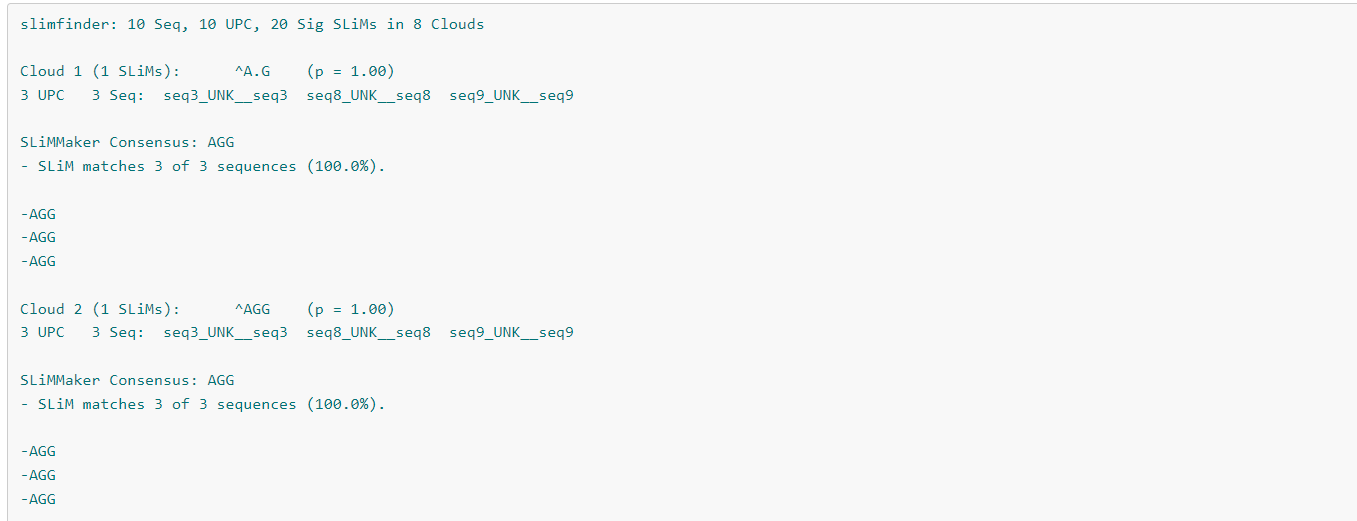
\includegraphics[width=14cm]{images/cloud1.png}
\end{center}
\begin{center}
\textbf{Generated Motif Part 1}
\end{center}
\vspace{8pt}

\vspace{8pt}
\begin{center}
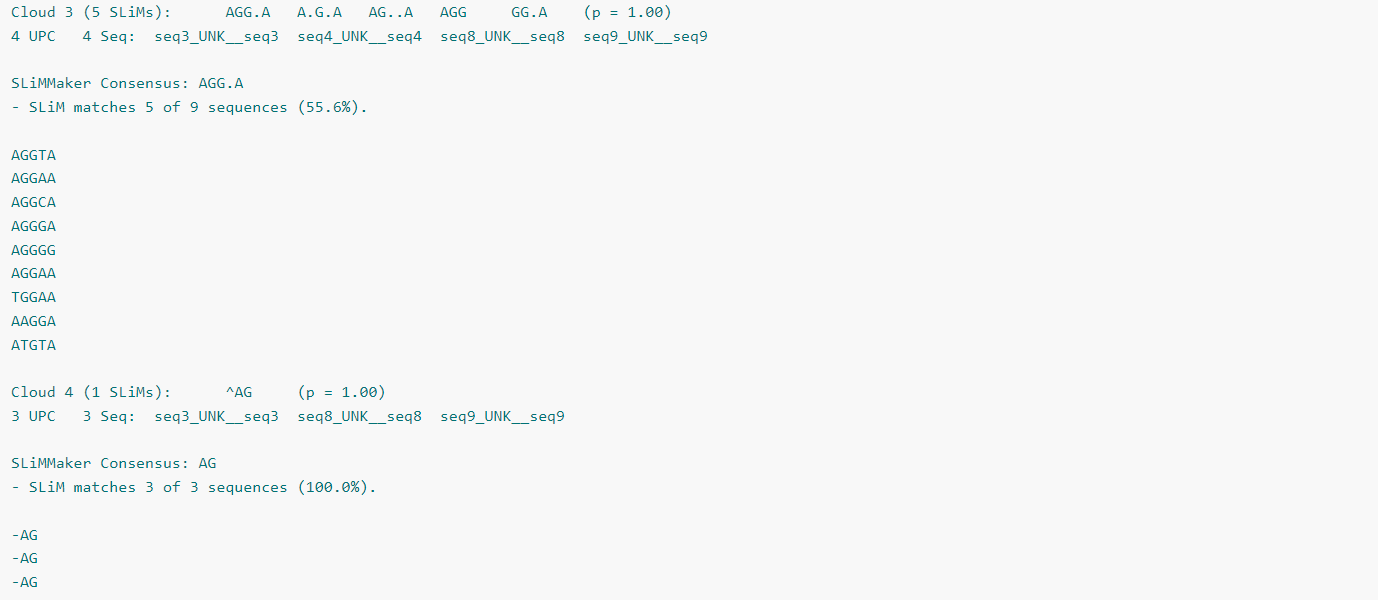
\includegraphics[width=14cm]{images/cloud2.png}
\end{center}
\begin{center}
\textbf{Generated Motif Part 2}
\end{center}
\vspace{8pt}

\vspace{8pt}
\begin{center}
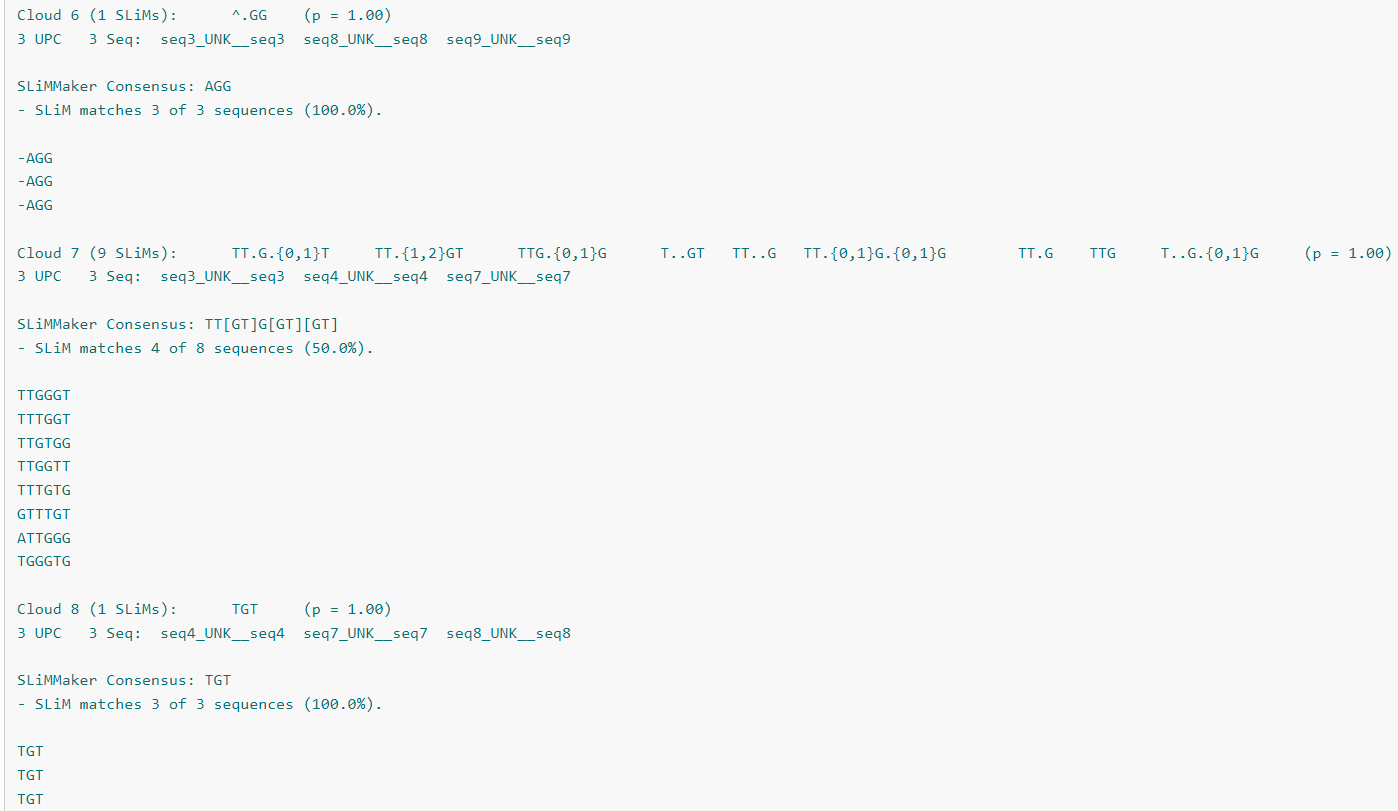
\includegraphics[width=14cm]{images/cloud3.png}
\end{center}
\begin{center}
\textbf{Generated Motif Part 3}
\end{center}
\vspace{8pt}

\vspace{8pt}
\begin{center}
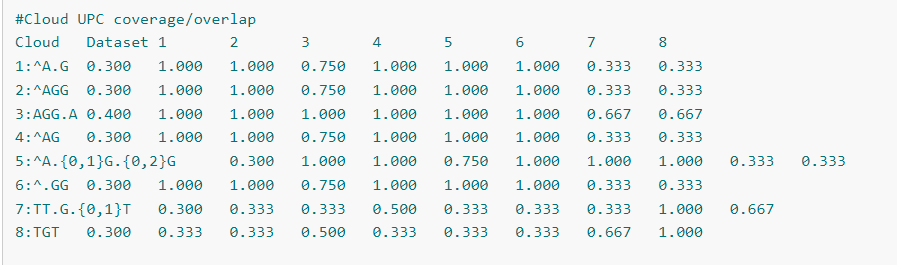
\includegraphics[width=14cm]{images/cloudOverlap.png}
\end{center}
\begin{center}
\textbf{Generated Motif Overlap Information}
\end{center}
\vspace{8pt}

The overlap information's helps us determine what part of the consensus are being matched. Also the generated motifs are being ranked based on their quality and precision.

\subsubsection{Portion of Generated Log}

\vspace{8pt}
\begin{center}
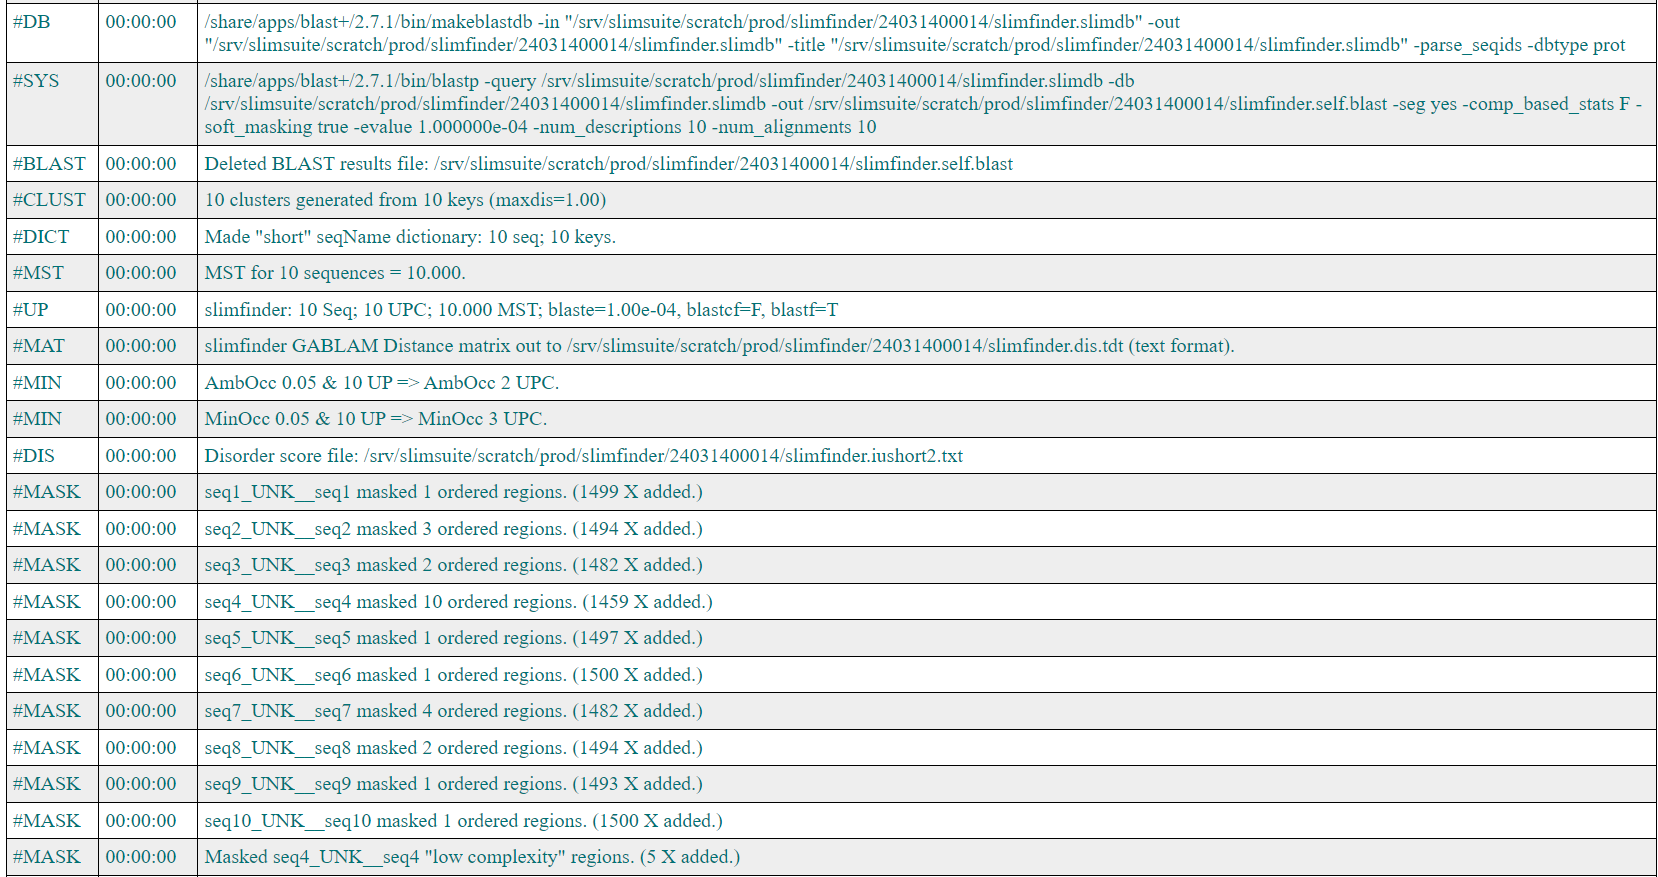
\includegraphics[width=14cm]{images/log1.png}
\end{center}
\begin{center}
\textbf{Generated Motif log part 1}
\end{center}
\vspace{8pt}

\vspace{8pt}
\begin{center}
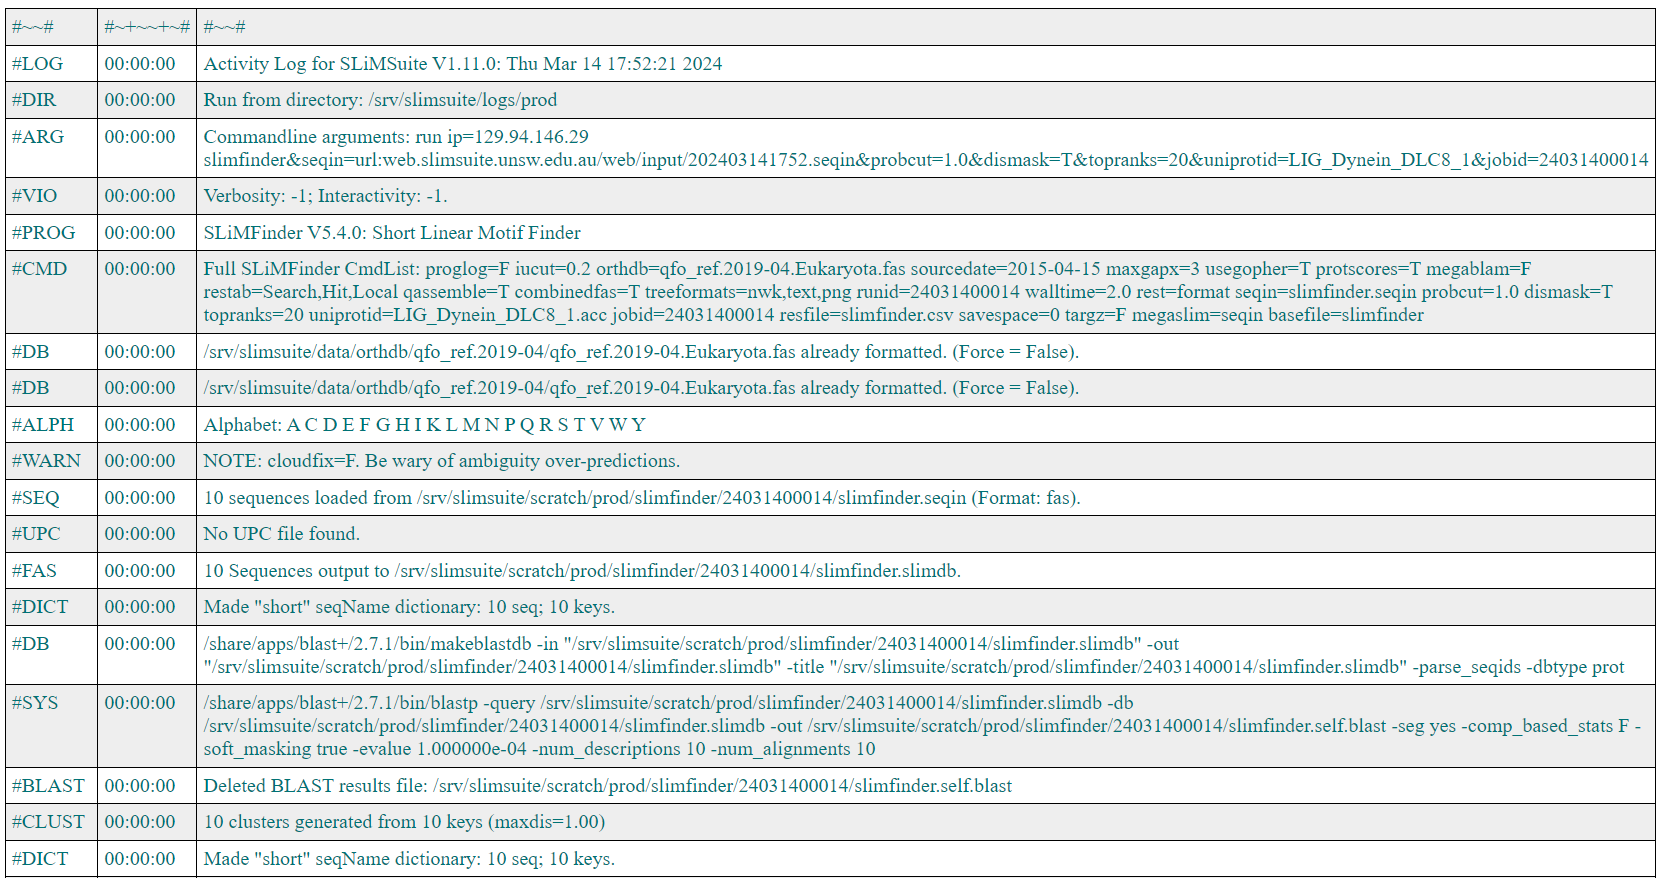
\includegraphics[width=14cm]{images/log2.png}
\end{center}
\begin{center}
\textbf{Generated Motif log part 2}
\end{center}
\vspace{8pt}

\subsubsection{Run Information}
The run information can be found here, these will be valid for 1 month:\\
\href{http://rest.slimsuite.unsw.edu.au/retrieve&jobid=24031400014&rest=format&password=None&refresh=4}{\textit{\textbf{Run Info of hm03, Human genome}}}
\\
\href{http://rest.slimsuite.unsw.edu.au/retrieve&jobid=24031400017&rest=format&password=None&refresh=4}{\textit{\textbf{Run Info of yst08r, Yeast}}}